\usetikzlibrary{shapes}
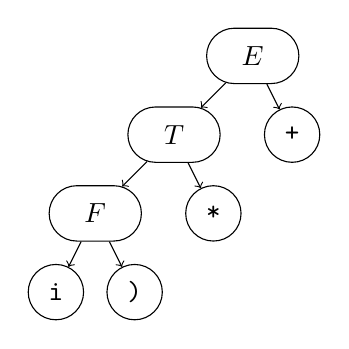
\begin{tikzpicture}
\tikzstyle{mono}=[draw,circle,minimum width=2em,font=\ttfamily];
\tikzstyle{con}=[draw,rounded rectangle,minimum height=2em,minimum width=4em];
\tikzstyle{dir}=[->];
\node [con] (v1) at (-1,0.5) {$E$};
\node [con] (v2) at (-2,-0.5) {$T$};
\node [con] (v3) at (-3,-1.5) {$F$};
\draw [dir] (v1) edge (v2);
\draw [dir] (v2) edge (v3);
\node [mono] (v6) at (-1.5,-1.5) {*};
\node [mono] (v4) at (-3.5,-2.5) {i};
\node [mono] (v5) at (-2.5,-2.5) {)};
\node [mono] (v7) at (-0.5,-0.5) {+};
\draw [dir] (v3) edge (v4);
\draw [dir] (v3) edge (v5);
\draw [dir] (v2) edge (v6);
\draw [dir] (v1) edge (v7);
\end{tikzpicture}